%%%%%%%%%%%%%%%%%%%%%%%%%%%%% Define Article %%%%%%%%%%%%%%%%%%%%%%%%%%%%%%%%%%
\documentclass{article}
%%%%%%%%%%%%%%%%%%%%%%%%%%%%%%%%%%%%%%%%%%%%%%%%%%%%%%%%%%%%%%%%%%%%%%%%%%%%%%%

%%%%%%%%%%%%%%%%%%%%%%%%%%%%% Using Packages %%%%%%%%%%%%%%%%%%%%%%%%%%%%%%%%%%
\usepackage[utf8]{inputenc}
\usepackage{float, geometry, graphicx, fancyhdr, color, xcolor}
\usepackage{amssymb, amsthm, amsmath, tikz, pgfplots, comment, wrapfig}
\usepackage{listings, mdframed, lipsum, psfrag, parskip, empheq, subfig, verbatim, pythonhighlight}
\usepackage[english]{babel}
\usepackage[breaklinks]{hyperref}
\usepackage{titlesec, cite, hyperref, wrapfig, booktabs, bookmark, pdfpages, lastpage, subfloat}
\usepackage{upgreek}
\usepackage{multirow}

%%%%%%%%%%%%%%%%%%%%%%%%%%%%%%%%%%%%%%%%%%%%%%%%%%%%%%%%%%%%%%%%%%%%%%%%%%%%%%%

%%%%%%%%%%%%%%%%%%%%%%%%%% C Code Listing Settings %%%%%%%%%%%%%%%%%%%%%%%%%%%%%%%%%%%%%%%
\definecolor{mGreen}{rgb}{0.25,0.63,0.15}
\definecolor{mGray}{rgb}{0.5,0.5,0.5}
\definecolor{mPurple}{rgb}{0.58,0,0.82}
\definecolor{codeBlue}{rgb}{0.01, 0.2, 0.92}
\definecolor{codegray}{rgb}{0.5,0.5,0.5}
\definecolor{codepurple}{rgb}{0.58,0,0.82}
\definecolor{codeblue}{rgb}{0.13,0.29,0.53}
\definecolor{backgroundColour}{rgb}{0.95,0.95,0.95}

\lstset{
    language=Python,
    backgroundcolor=\color{backgroundColour},
    basicstyle=\ttfamily\small,
    commentstyle=\color{deepGreen},
    keywordstyle=\color{blue},
    numberstyle=\tiny\color{mGray},
    stringstyle=\color{red},
    breakatwhitespace=false,         
    breaklines=true,                 
    captionpos=b,                    
    keepspaces=true,                 
    numbers=left,                    
    numbersep=5pt,                  
    showspaces=false,                
    showstringspaces=false,
    showtabs=false,                  
    tabsize=2,
    frame=single
}

%%%%%%%%%%%%%%%%%%%%%%%%%%%%%%%%%%%%%%%%%%%%%%%%%%%%%%%%%%%%%%%%%%%%%%%%%%%%%%%

% Other Settings
\hypersetup{
    colorlinks = true,
    linkcolor = black,
    urlcolor = blue,
}
\urlstyle{same}

%%%%%%%%%%%%%%%%%%%%%%%%%% Page Setting %%%%%%%%%%%%%%%%%%%%%%%%%%%%%%%%%%%%%%%
\geometry{a4paper}
\pagestyle{fancy}
\fancyhead{}
\fancyhead[L]{SQL Report}
\fancyhead[C]{Data Science Internsip}
\fancyhead[R]{10Pearls}
\fancyfoot{}
\fancyfoot[C]{\thepage \;of \pageref{LastPage}}

%%%%%%%%%%%%%%%%%%%%%%%%%% Define some useful colors %%%%%%%%%%%%%%%%%%%%%%%%%%
\definecolor{ocre}{RGB}{243,102,25}
\definecolor{mygray}{RGB}{243,243,244}
\definecolor{deepGreen}{RGB}{26,111,0}
\definecolor{shallowGreen}{RGB}{235,255,255}
\definecolor{deepBlue}{RGB}{61,124,222}
\definecolor{shallowBlue}{RGB}{235,249,255}
%%%%%%%%%%%%%%%%%%%%%%%%%%%%%%%%%%%%%%%%%%%%%%%%%%%%%%%%%%%%%%%%%%%%%%%%%%%%%%%

%%%%%%%%%%%%%%%%%%%%%%%%%% Define an orangebox command %%%%%%%%%%%%%%%%%%%%%%%%
\newcommand\orangebox[1]{\fcolorbox{ocre}{mygray}{\hspace{1em}#1\hspace{1em}}}
%%%%%%%%%%%%%%%%%%%%%%%%%%%%%%%%%%%%%%%%%%%%%%%%%%%%%%%%%%%%%%%%%%%%%%%%%%%%%%%

%%%%%%%%%%%%%%%%%%%%%%%%%%%% English Environments %%%%%%%%%%%%%%%%%%%%%%%%%%%%%
\newtheoremstyle{mytheoremstyle}{3pt}{3pt}{\normalfont}{0cm}{\rmfamily\bfseries}{}{1em}{{\color{black}\thmname{#1}~\thmnumber{#2}}\thmnote{\,--\,#3}}
\newtheoremstyle{myproblemstyle}{3pt}{3pt}{\normalfont}{0cm}{\rmfamily\bfseries}{}{1em}{{\color{black}\thmname{#1}~\thmnumber{#2}}\thmnote{\,--\,#3}}
\theoremstyle{mytheoremstyle}
\newmdtheoremenv[linewidth=1pt,backgroundcolor=shallowGreen,linecolor=deepGreen,leftmargin=0pt,innerleftmargin=20pt,innerrightmargin=20pt,]{theorem}{Theorem}[section]
\theoremstyle{mytheoremstyle}
\newmdtheoremenv[linewidth=1pt,backgroundcolor=shallowBlue,linecolor=deepBlue,leftmargin=0pt,innerleftmargin=20pt,innerrightmargin=20pt,]{definition}{Definition}[section]
\theoremstyle{myproblemstyle}
\newmdtheoremenv[linecolor=black,leftmargin=0pt,innerleftmargin=10pt,innerrightmargin=10pt,]{problem}{Problem}[section]
%%%%%%%%%%%%%%%%%%%%%%%%%%%%%%%%%%%%%%%%%%%%%%%%%%%%%%%%%%%%%%%%%%%%%%%%%%%%%%%

\title{{\huge \textbf{10Pearls Data Science Internship}}

% \vspace*{5mm}
{\LARGE \textbf{SQL Analysis Report}} \\ \vspace*{2mm}
% {
\includegraphics[width=0.60\linewidth]{../assets/10p_logo.jpeg}}
}
\author{Ali Muhammad Asad - aa07190}
\date{}

\pgfplotsset{compat=1.18}

\begin{document}
\maketitle

% \newpage
\tableofcontents

\newpage
\section{Introduction}
This report presents the findings, insights and analysis of a SQL analysis conducted as part of the Data Science Internship at 10Pearls. The primary objective of this analysis is to explore and understand customer behavior patterns by leveraging a well-structured SQL database and schema.

By analyzing various aspects of customer information, services, and billings, this report aims to provide actionable recommendations that can enhance customer engagement and drive business growth. 

The Telco Customer Churn data was first processed to drop the Churn values, make predictions based on the machine learning model, and then a schema was designed to store the data in a structured manner. The SQL database was then created on PostgreSQL and the schema was implemented.

\newpage
\section{Database and Schema Design}
The database was designed to store the Telco Customer Churn data in a structured manner. The schema was designed to store the data in a normalized form to ensure data integrity and reduce redundancy. The schema design is as follows:
\begin{figure}[h]
    \centering
    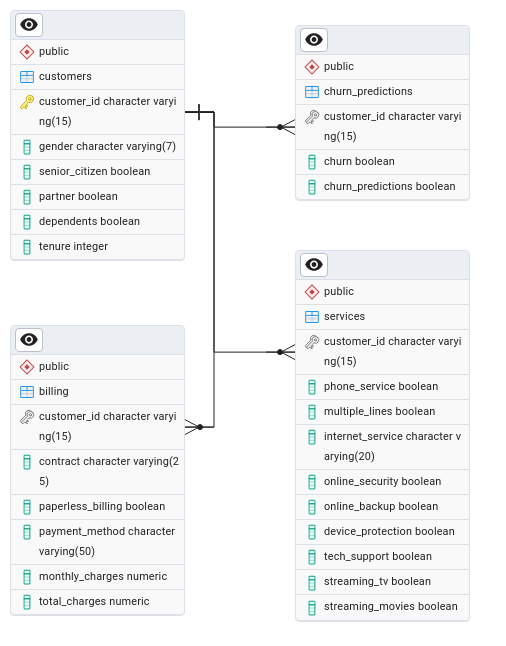
\includegraphics[width=0.8\linewidth]{../assets/schema.png}
    \caption{Database Schema}
\end{figure}

\newpage
\section{Analysis from the Data}
The analysis was conducted by querying the database using SQL queries. The following sections present the key findings and insights from the analysis.
\subsection{Tenure}
By executing queries on tenures, we were able to generate the following insights:
\begin{itemize}
    \item The longest tenure was of 72 months (6 years) and 362 customers had this tenure, while only 1 customer was predicted to churn amongst them. 
    \item The shortest tenure was of only 1 month and 613 customers had this tenure, while 463 of them were predicted to churn.
    \item 2058 customers have had a tenure of less than 1 year, 117 customers have had a tenure of exactly 1 year, and 4857 customers have had a tenure of more than 1 year.
    \item From those who's tenure was less than 1 year, 1129 were predicted to churn.
    \item The average tenure has been about 32 months (2 years and 8 months).
\end{itemize}

\subsection{Monthly Charges}
By executing queries on monthly charges, we were able to generate the following insights:
\begin{itemize}
    \item The highest monthly charges were \$118.75 of only one customer, who was availing all the services.
    \item The lowest monthly charges were \$18.25 of only one customer, who was only availing one service (Phone Service).
    \item The average monthly charges were \$64.8 (\$65 rounded up).
    \item 3130 customers are billed less than or equal to the average charges, while the remaining 3902 are billed more than the average charges.
\end{itemize}

\subsection{Total Charges}
By executing queries on total charges, we were able to generate the following insights:
\begin{itemize}
    \item The highest total charges were \$8684.8 of only one customer, who was availing all the services, paying a high monthly charge of \$117.8, having a tenure of 72 months, a 1 year contract, and was predicted to churn.
    \item The lowest total charges were \$18.8 of only one customer, who was only availing one service (Phone Service), paying a low monthly charge of \$18.8, having a tenure of 1 month, a 1 year contract, and was predicted not to churn.
    \item The average total charges were \$2283.3 (\$2300 rounded up).
    \item 4397 customers are being billed less than or equal to the average, while the remaining 2635 customers are paying more than the average.
\end{itemize}

\subsection{Contracts}
The table below summarizes the analysis of contracts (the churn values and churn rates are predicted churn rates - predictions made from our machine learning model):

\begin{table}[H]
    \centering
    \begin{tabular}{|c|c|c|c|c|c|c|}
        \hline
        \textbf{Contract} & \textbf{\# Customers} & \textbf{Avg Monthly \$} & \textbf{Avg Total \$} & \textbf{\# Churned} & \textbf{Churn Rate (\%)} \\
        \hline
        Month-to-Month & 3875 & 66.4 & 1369.25 & 1682 & 43.40 \\
        One Year & 1472 & 65.07 & 3034.68 & 149 & 10.12 \\
        Two Year & 1685 & 60.87 & 3728.93 & 32 & 1.90 \\
        \hline
    \end{tabular}
    \caption{Analysis of Contracts}
\end{table}

We can infer the following insights from the analysis:
\begin{itemize}
    \item Month-to-Month contracts have the highest predicted churn rate of 43.4\% with 1682 customers predicted to churn out of 3875, they also have the highest average monthly charges of \$66.4 and the lowest average total charges of \$1369.25 (which might be due to the high churn rate, hence their total charges don't cumulate much).
    \item Month-to-Month contracts also have the highest number of customers.
    \item Two Year contracts have the lowest predicted churn rate of 1.90\% with 32 customers predicted to churn out of 1685, while having the lowest average monthly charges of \$60.87, yet still having a considerable amount of customers.
    \item One Year contracts have a moderate predicted churn rate of 10.12\% with 149 customers predicted to churn out of 1472, having an average monthly charge of \$65.07 and an average total charge of \$3034.68.
\end{itemize}


\subsection{Payment Methods}
The table below summarizes the analysis of payment methods (the churn values and churn rates are predicted churn rates - predictions made from our machine learning model):

\begin{table}[H]
    \centering
    \begin{tabular}{|c|c|c|c|c|c|c|}
        \hline
        \textbf{Payment Method} & \textbf{\# Customers} & \textbf{Avg Monthly \$} & \textbf{Avg Total \$} & \textbf{\# Churned} & \textbf{Churn Rate (\%)} \\
        \hline
        Bank Transfer & 1542 & 67.21 & 3079.30 & 238 & 15.43 \\
        Credit Card & 1521 & 66.52 & 3071.40 & 218 & 14.33 \\
        Electronic Check & 2365 & 76.26 & 2090.90 & 1103 & 46.64 \\
        Mailed Check & 1604 & 43.96 & 1054.48 & 304 & 18.95 \\
        \hline
    \end{tabular}
    \caption{Analysis of Payment Methods}
\end{table}

We can infer the following insights from the analysis:

\begin{itemize}
    \item Electronic Check payment method has the highest predicted churn rate of 46.64\% with 1103 customers predicted to churn, they also have the highest average monthly charges of \$76.26 and the lowest average total charges of \$2090.90 (again which might be due to high churn rate).
    \item Credit Card (Automatic) payment method has the lowest predicted churn rate of 14.33\% with 218 customers predicted to churn out of 1521, they also have the second highest average monthly charges of \$66.52 and the second highest average total charges of \$3071.40, but also have the least number of customers.
\end{itemize}


\subsection{Services}
The table below summarizes the analysis of services (the churn values and churn rates are predicted churn rates - predictions made from our machine learning model):

\begin{table}[H]
    \centering
    \begin{tabular}{|c|c|c|c|c|c|c|}
        \hline
        \textbf{Internet Service} & \textbf{\# Customers} & \textbf{Avg Monthly \$} & \textbf{Avg Total \$} & \textbf{\# Churned} & \textbf{Churn Rate (\%)} \\
        \hline
        DSL & 2416 & 58.09 & 2119.79 & 447 & 18.50 \\
        No Service & 1520 & 21.08 & 665.22 & 108 & 7.10 \\
        Fiber Optic & 3096 & 91.5 & 3205.30 & 1308 & 42.24 \\
        \hline
    \end{tabular}
    \caption{Analysis of Services}
\end{table}

We can infer the following insights from the analysis:

\begin{itemize}
    \item Fiber Optic internet service has the highest predicted churn rate of 42.24\% with 1308 customers predicted to churn, they also have the highest average monthly charges of \$91.5 and the highest average total charges of \$3205.30 which may suggest that the fiber optic service might not be upto the mark and the customers are not satisfied with it.
    \item Customers without any internet service have the lowest predicted churn rate of 7.10\% with 108 customers predicted to churn out of 1520, they also have the lowest average monthly charges of \$21.08 and the lowest average total charges of \$665.22.
\end{itemize}


\subsection{General Stuff}
\begin{itemize}
    \item All the customers who do not use any phone service only use DSL as their internet service which has a 15.31\% churn prediction rate.
    \item The total revenue generated was \$16056168.70.
    \item The total revenue generated by predicted churned customers was \$2862926.90.
\end{itemize}

Predicted Churned Averages:

\begin{table}[H]
    \centering
    \begin{tabular}{|c|c|c|c|c|}
        \hline
        \textbf{Churn Prediction} & \textbf{\# Customers} & \textbf{Avg Monthly \$} & \textbf{Avg Total \$} \\
        \hline
        False & 5169 & 61.39 & 2580.71 \\
        True & 1863 & 74.26 & 1458.11 \\
        \hline
    \end{tabular}
    \caption{Predicted Churned Averages}
\end{table}


\newpage
\section{Advanced Analysis - Trends, Running Totals and Averages}
\subsection{Churn Patterns by Tenure}
It was found that the people with the shortest tenures are most likely to churn, as per predictions. It is interesting that the first 5 months have the highest churn rates in that order. The table below shows the churn rates by tenure:

\begin{table}[H]
    \centering
    \begin{tabular}{|c|c|c|}
        \hline
        \textbf{Rank} & \textbf{Tenure (Months)} & \textbf{Churn Count} \\ 
        \hline
        1 & 1 & 383 \\
        2 & 2 & 129 \\
        3 & 3 & 101 \\
        4 & 4 & 90 \\
        5 & 5 & 58 \\
        \hline
    \end{tabular}    
    \caption{Churn Patterns by Tenure}
\end{table}

\subsection{Running Total and Moving Average on Monthly Charges}
The following two images depict the running total, and moving average charges over monthly charges respectively.

\begin{figure}[h]
    \centering
    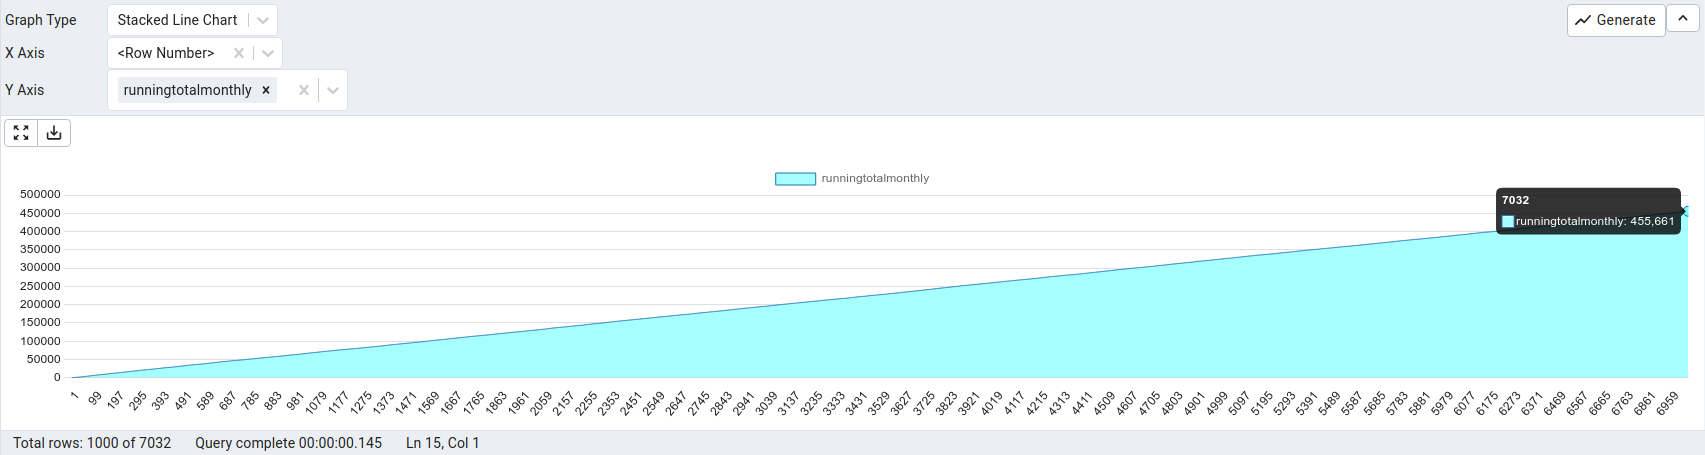
\includegraphics[width=\textwidth]{running_total_monthly.png}
    \caption{Running Total on Monthly Charges}

    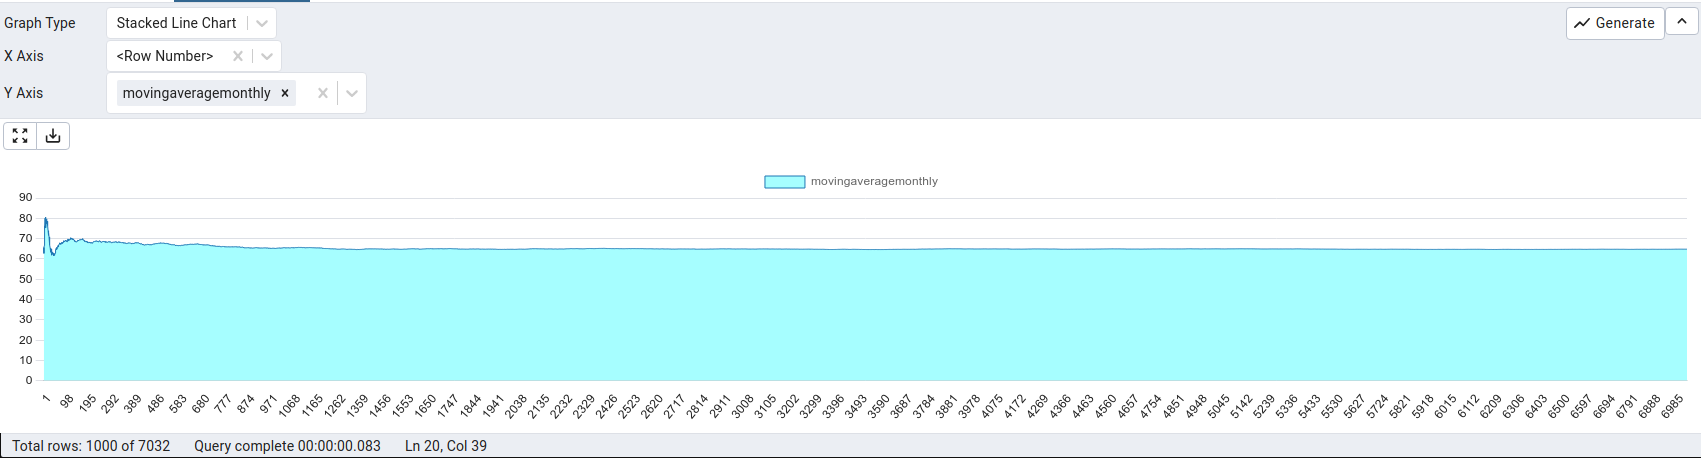
\includegraphics[width=\textwidth]{moving_average_monthly.png}
    \caption{Moving Average on Monthly Charges}
\end{figure}

\subsection{Running Total and Moving Average on Total Charges}
The following two images depict the running total, and moving average charges over total charges respectively.

\begin{figure}[h]
    \centering
    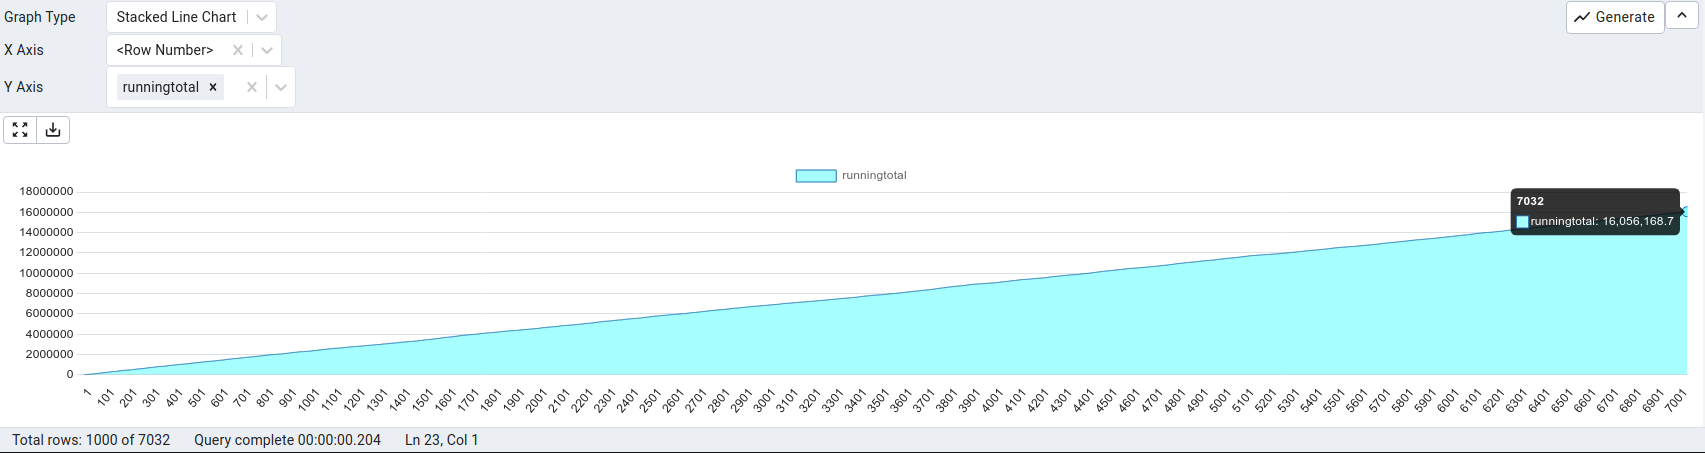
\includegraphics[width=\textwidth]{running_total.png}
    \caption{Running Total on Total Charges}

    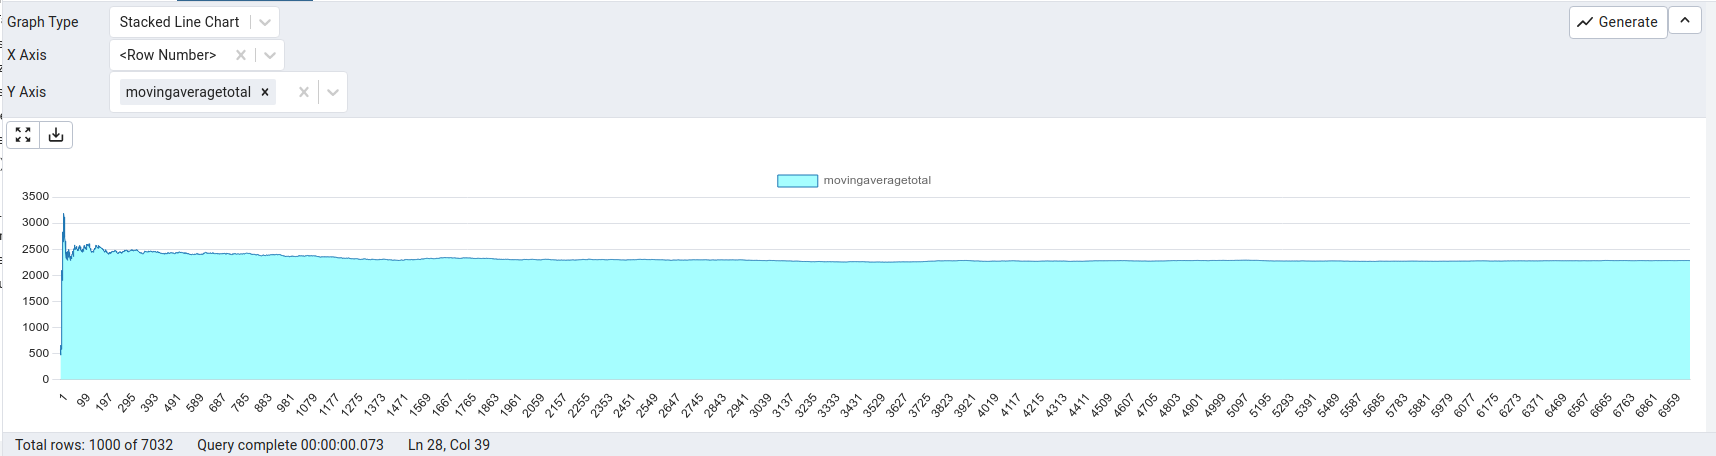
\includegraphics[width=\textwidth]{moving_average_total.png}
    \caption{Moving Average on Total Charges}
\end{figure}

\end{document}
